\section{Full Battery and Confidence Intervals}
\label{app:battery}

Table~\ref{tab:fullbattery} gives every condition with Wilson $95\%$ intervals
($N = 400$). Base A1/A2/D1 are not in our committed data and are omitted rather than
estimated.

\begin{table}[h]
\centering
\footnotesize
\setlength{\tabcolsep}{3pt}
\begin{tabular}{@{}llcc@{}}
\toprule
 & surface & base & instruct \\
\midrule
C0 & \texttt{B * C =} & .838\,{\scriptsize[.80,.87]} & .848\,{\scriptsize[.81,.88]} \\
C1 & \texttt{( 0 + B ) * C =} & .508\,{\scriptsize[.46,.56]} & .265\,{\scriptsize[.22,.31]} \\
C2 & \texttt{( 0 + B * C ) =} & n/a & .678\,{\scriptsize[.63,.72]} \\
C3 & \texttt{( B ) * C =} & n/a & .755\,{\scriptsize[.71,.80]} \\
C4 & \texttt{( B * C ) =} & .890\,{\scriptsize[.86,.92]} & .908\,{\scriptsize[.88,.93]} \\
C5 & \texttt{0 + B * C =} & n/a & .542\,{\scriptsize[.49,.59]} \\
C6 & \texttt{( 0 + B ) =} & 1.00\,{\scriptsize[.99,1.0]} & 1.00\,{\scriptsize[.99,1.0]} \\
C7 & \texttt{(0+B)*C=} & .018\,{\scriptsize[.01,.04]} & .190\,{\scriptsize[.16,.23]} \\
C8 & \texttt{(B*C)=} & .765\,{\scriptsize[.72,.80]} & .785\,{\scriptsize[.74,.82]} \\
A1 & \texttt{( 0 + B ) + C =} & n/a & .995\,{\scriptsize[.98,1.0]} \\
A2 & \texttt{0 + ( B + C ) =} & n/a & .928\,{\scriptsize[.90,.95]} \\
D1 & \texttt{(( 0 + B )) * C =} & n/a & .038\,{\scriptsize[.02,.06]} \\
\bottomrule
\end{tabular}
\caption{Full battery, exact-match accuracy with Wilson $95\%$ CIs.}
\label{tab:fullbattery}
\end{table}

\paragraph{Magnitude control.} Within matched $|B\!\cdot\!C|$ bins (instruct), C1 vs C4:
$[440,813)$ .53/.96 ($n{=}79$); $[813,1185)$ .28/.94 (126); $[1185,1558)$ .16/.89 (104);
$[1558,1930)$ .19/.89 (64); $[1930,2303)$ .00/.70 (27). Every paired difference has a
positive bootstrap CI.

\section{Wrapper Blind-Spot Map}
\label{app:wrapper}
\begin{figure}[h]
\centering
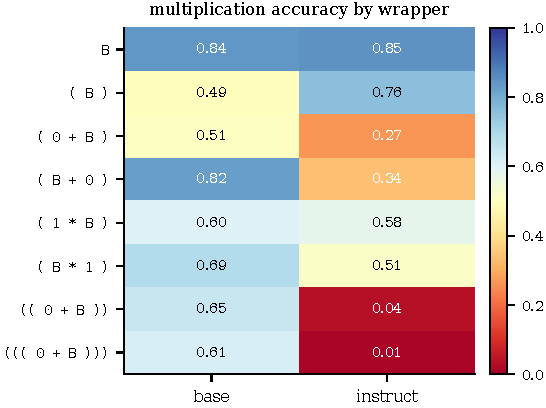
\includegraphics[width=0.82\columnwidth]{figs/figA_wrapper.pdf}
\caption{Multiplication accuracy by wrapper. Position-dependence is a base-model effect
(left-placed $(\,0{+}B\,)$ collapses, right-placed $(\,B{+}0\,)$ barely moves; instruct degrades
on both placements), and instruction tuning is not uniformly worse (plain parentheses).}
\label{fig:wrapper}
\end{figure}

\section{By-Layer Decodability}
\label{app:decode}
\begin{figure}[h]
\centering
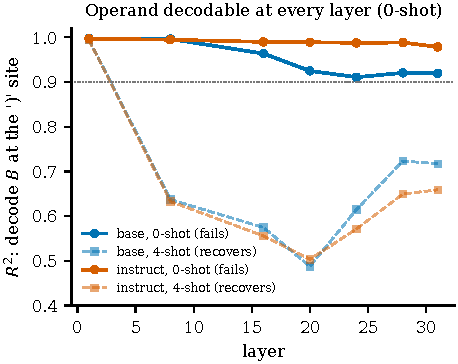
\includegraphics[width=0.82\columnwidth]{figs/figA_decode.pdf}
\caption{Operand $B$ decodes at every layer in the failing zero-shot regime (solid). The
few-shot curves (dashed) drop mid-network; shown for completeness only, and we draw no
mechanistic conclusion from the few-shot decodability.}
\label{fig:decode}
\end{figure}

\section{Steering Nulls}
\label{app:steering}
\begin{figure}[h]
\centering
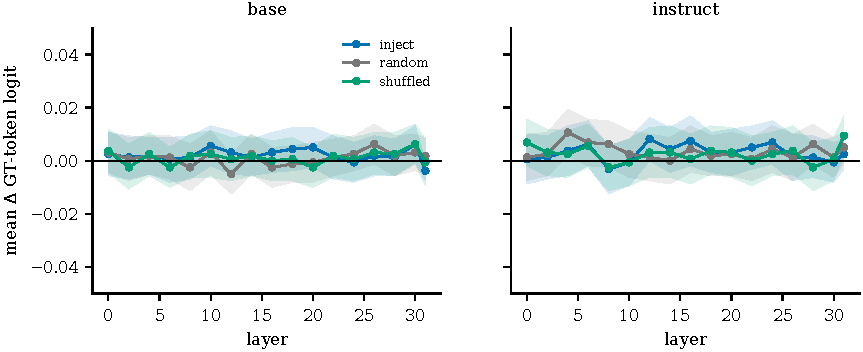
\includegraphics[width=\columnwidth]{figs/figA_steering.pdf}
\caption{Probe-direction steering at ``$=$'' is inert at every layer for inject, random,
and shuffled targets (mean $\Delta$ ground-truth-token logit, $95\%$ CIs through zero).
This first-token metric is a null; the discriminative full-product re-score is
Figure~\ref{fig:evidence}b.}
\label{fig:steernull}
\end{figure}

\section{Cross-Model Battery}
\label{app:crossmodel}
Matched bare format, in scope if C4 and C6 $\geq 0.80$: Llama-3.1-8B base C1 $.508$ /
instruct $.265$; Gemma-2-9b-it $.043$ (C4 $.99$); Llama-3.2-3B $.358$ (C4 $.88$). Out of
scope (parts fail): Qwen2.5-7B (C4 $.00$), Mistral-7B (C4 $.62$), Llama-3.2-1B (C4 $.31$).
Chat format: Gemma-2-9b-it composes (C1 $.95$, C4 $.99$) but Llama-3.1-8B chat falls out of
scope (C4 $.70$); the composing and failing models are never in the same format.
